\chapter{Spherical harmonics}\label{app:SH}
The (tesseral) spherical harmonic function of degree $n$ and order $m$ 
($n\in\mathbb{N}_0,\ m\in\mathbb{Z}, 0\leq \abs{m} \leq n$) is defined as (\cite[Sec. 3.13]{Schreiner})
\begin{equation}\label{eq:Ynm}
\nomenclature[a]{$\Y{n}{m}$}{spherical harmonic function of degree $n$ and order $m$\nomrefeq}
\nomenclature[a]{$\kron{i}{j}$}{Kronecker delta symbol ($\kron{i}{j} = 1$ if $i = j$ and $\kron{i}{j} = 0$ otherwise}
    \Y{n}{m}(\bomega) = \Y{n}{m}(\polar,\azimuthal) = 
    \sqrt{(2-\delta_{m0})\frac{2n+1}{4\pi}\frac{(n-\abs{m})!}{(n+\abs{m})!}} \P{n}{\abs{m}}(\cos\polar)T_m(\azimuthal),
\end{equation}
or, if we denote $\mu = \cost$\nomenclature[g]{$\mu$}{cosine of the polar component of the direction vector $\bomega$} 
the cosine of the polar component of the direction vector $\bomega$ (see \fref{fig:scatter}),
$$
	\sqrt{(2-\kron{m}{0})\frac{2n+1}{4\pi}\frac{(n-\abs{m})!}{(n+\abs{m})!}} \P{n}{\abs{m}}(\mu)T_m(\azimuthal);
$$
$\kron{i}{j} = 1$ if $i = j$ and $\kron{i}{j} = 0$ otherwise is the Kronecker delta symbol,
\begin{equation}
\label{eq:associated_Pn}
    \nomenclature[a]{$\P{n}{m}(\mu)$}{associated Legendre polynomial of degree $n$ and order $m$\nomrefeq} 
    \P{n}{m}(\mu) = \sqrt{(1-\mu^2)^m}\ \der[m]{\P{n}{}(\mu)}{\mu}, \quad m > 0
\end{equation}
are the \textit{associated Legendre functions},
$$
T_{m}(\azimuthal) = 
    \begin{cases} 
    	\cos m\azimuthal & m \geq 0 ,\\
    	\sin \abs{m}\azimuthal & m < 0 
    \end{cases}
$$
and $\P{n}{}(\mu) = \P{n}{0}(\mu)$ is the $n$-th member of the system of Legendre polynomials:
\begin{equation}\label{eq:leg}
\nomenclature[a]{$\P{n}{}(\mu)$}{Legendre polynomial of degree $n$}\nomrefeq
\begin{gathered}
	\P{0}{}(\mu) = 1,\quad \P{1}{}(\mu) = \mu,\quad \P{2}{}(\mu) = \frac12(3\mu^2 - 1),
\quad \P{3}{}(\mu) = \frac12(5\mu^3 - 3\mu)\\
 	(2n + 1)\mu\P{n}{}(\mu) = (n+1)\P{n+1}{}(\mu) + n\P{n-1}{}(\mu), \quad n = 1,2,\ldots
\end{gathered}
\end{equation}

Spherical harmonics form a complete orthonormal system on $\Lp[2](\Sphere)$ with respect to the
standard inner product $$
(\psi, \varphi)_{\Lp[2](\Sphere)} = \intA{\psi(\bomega) {\varphi(\bomega)}},
$$
that is
\begin{equation}\label{eq:og}
\begin{aligned}
\intA{\Y{n}{m}(\bomega)\Yc{n}{m}(\bomega)} &=
\int_{0}^{2\pi}\d{\azimuthal}\int_{0}^{\pi}\sin\polar\d{\polar}  
\Y{n}{m}(\polar,\azimuthal)\Yc{l'}{m'}(\polar,\azimuthal)\\[.25em]
& = \int_{0}^{2\pi}\d{\azimuthal}\int_{-1}^{1}\d{\mu}
\Y{n}{m}(\mu,\azimuthal)\Yc{l'}{m'}(\mu,\azimuthal) = \kron{n}{l'}\kron{m}{m'}
\end{aligned}
\end{equation}
Similarly, Legendre polynomials form a complete orthogonal system on the interval $[-1,1]$:
$$
	\muint {\P{n}{}(\mu)\P{m}{}(\mu)} = \frac{2\kron{n}{m}}{2n + 1}.
$$

Spherical harmonics satisfy the
following \textit{addition theorem} (e.g., \cite[Remark 3.88]{Schreiner}), which allows to express the value of Legendre
polynomial of degree $k$ at $\mu_0 = \cos\polar_0 = \bomega\cdot\bomega'$ (\fref{fig:scatter}) as a dot product of
vectors with values of the $2n+1$ spherical harmonics at $\bomega$ and $\bomega'$, respectively:
\begin{align}
\P{n}{}(\mu_0)
&=P_n(\mu) P_n(\mu')+2 \sum _{m = 1}^n \frac{(n-m)!}{(n+m)!} \cos \bigl(m(\azimuthal - \azimuthal')\bigr) P_n^m(\mu) P_n^m(\mu')\nonumber\\
&=\frac{4\pi}{2n+1}\suma[m]{-n}{n}\Y{n}{m}(\polar,\azimuthal)\Yc{n}{m}(\polar',\azimuthal'),
\label{eq:additionThm}
\end{align}
Note that this greatly simplifies integrals of type
$$
\intA[']{P_n(\bomega\cdot\bomega')f(\bomega')}
$$
(as in the proof of Lemma \ref{lem:appC}), because of the complicated form of $\bomega\cdot\bomega'$:
$$
\begin{aligned}
	\bomega\cdot\bomega' 
&= \lvect{\sint\cosp,\sint\sinp,\cost} \cdot \lvec{\sint'\cosp',\sint'\sinp',\cost'} \\
& = \mu'\mu + \sqrt{(1-\mu'^2)(1-\mu^2)}\cos(\azimuthal' - \azimuthal),
\end{aligned}
$$
\begin{figure}[!hbt]
    \centering
    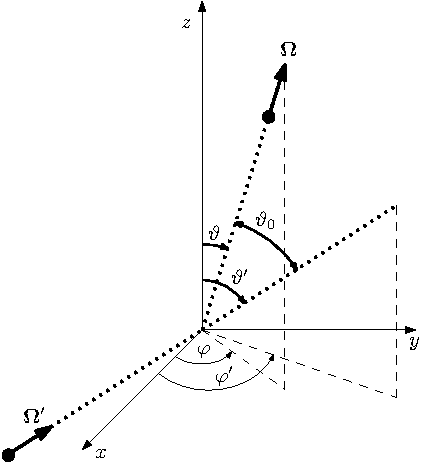
\includegraphics[scale=1.65]{scattering.eps}
    \caption[Scattering]{Geometry of scattering}
    \label{fig:scatter}
\end{figure}

Linear combination of spherical
harmonics of degree $n$ produces a \textit{surface spherical harmonic of degree $n$}:
\begin{equation*}
\begin{multlined}
    \mathcal{Y}_n(\bomega) = \mathcal{Y}_n(\polar,\azimuthal) = \\A_0 P_n(\cos\polar) + \suma[m]{1}{n}\left[ A_m
    \cos(m\azimuthal)\P{n}{m}(\cos\polar) + B_m \sin(m\azimuthal)\P{n}{m}(\cos\polar)\right]
  \end{multlined}
  \end{equation*}
Surface spherical harmonics are formally defined as restrictions of homogeneous harmonic polynomials of degree $n$ to
unit sphere $\Sphere$ (\cite[Art. 110]{Byerly}, \cite[Def. 3.22]{Schreiner}).

\comment{
\newpage
\begin{sidewaysfigure}
	\centering
		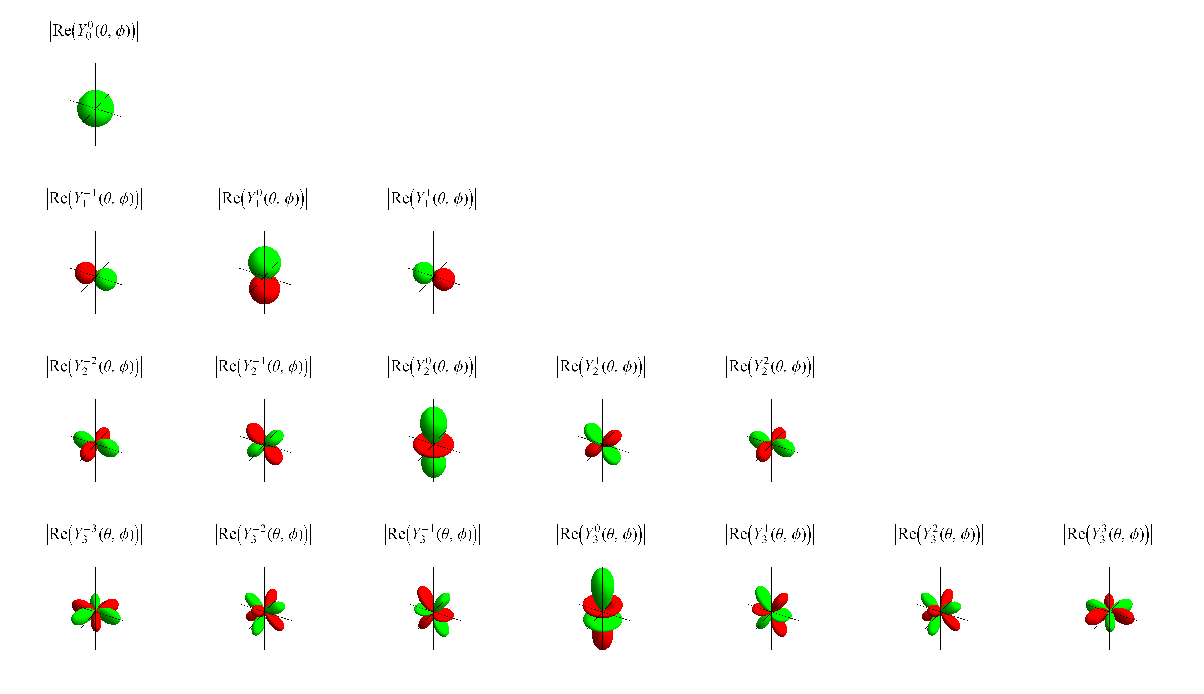
\includegraphics[scale=1.2]{pic/sh.eps}
		\caption[Spherical harmonics]{Spherical harmonics up to $3^{\mbox{rd}}$ degree, plotted in spherical coordinates 
		as specified in the labels above the graphs and colored green if $\Y{n}{m} \geq 0$ and red
		otherwise.}%
	\label{fig:SH} 
\end{sidewaysfigure}
}


